\documentclass[UTF8,a4paper]{ctexart}
\usepackage[margin=1in]{geometry}
\usepackage{graphicx,float,array,color,bm,amsmath,amssymb,hyperref}
\pdfstringdefDisableCommands{\let\bm\@firstofone}
\hypersetup{hidelinks}
\author{qhy}
\date{\today}
\title{Gaussian Process}
\begin{document}
    \maketitle
    \tableofcontents
    \newpage
    \section{Gaussian Process}
        \subsection{数学基础}
        在GP中需要用到的数学知识,这里给出结论,证明见PRML第二章。
            \subsubsection{高斯分布}
            给定一个联合高斯分布$\mathcal{N}(\bm{x}|\bm{\mu,\Sigma})$,其中$\bm{\Lambda} \equiv \bm{ \Sigma^{-1}}$,且
            \begin{equation}
                \bm{x} = \left ( \begin{array}{l}
                \bm{x_a} \\
                \bm{x_b}
                \end{array}
                \right ),
                \bm{\mu} = \left ( \begin{array}{l}
                \bm{\mu_a} \\
                \bm{\mu_b}
                \end{array}
                \right )
            \end{equation}
            \begin{equation}
                \bm{\Sigma} = \left (
                \begin{array}{cc}
                \bm{\Sigma_{aa}} & \bm{\Sigma_{ab}}\\
                \bm{\Sigma_{ba}}& \bm{\Sigma_{bb}}
                \end{array} \right ),
                \bm{\Lambda} = \left (
                \begin{array}{cc}
                \bm{\Lambda_{aa}} & \bm{\Lambda_{ab}}\\
                \bm{\Lambda_{ba}}& \bm{\Lambda_{bb}}
                \end{array}\right )
            \end{equation}

            有以下两个结论:

            \textbf{条件概率分布:}
            \begin{equation}
                p(\bm{x_a}|\bm{x_b}) = \mathcal{N}(\bm{x_a}|\bm{\mu_{a|b}},\bm{\Lambda_{aa}^{-1}})
            \end{equation}
            \begin{equation}
                \bm{\mu_{a|b}} = \bm{\mu_a} - \bm{\Lambda_{aa}^{-1}\Lambda_{ab}(x_b - \mu_b)}
            \end{equation}
            或
            \begin{equation}
                \bm{\mu_{a_b}} = \bm{\mu_a + \Sigma_{ab}\Sigma_{bb}^{-1}(x_b - \mu_a)}
            \end{equation}
            \begin{equation}
                \bm{\Sigma_{a|b}= \Sigma_{aa} - \Sigma_{ab}\Sigma_{bb}^{-1}\Sigma_{ba}}
            \end{equation}

            \textbf{边缘概率分布:}
            \begin{equation}
                p(\bm{x_a}) = \mathcal{N}(\bm{x_a|\mu_a,\Sigma_{aa}})
            \end{equation}

            {\color{blue}这里证明了边缘概率和联合分布之间的关系,当我们在求边缘概率的时候,就可以通过求联合分布得到(这里在计算的时候省略的积分的过程,但实际的证明就是通过积分证明得到的。)}

            \subsubsection{高斯变量的贝叶斯定理}

            给定$\bm{x}$的一个边缘高斯分布,以及在给定$\bm{x}$的条件下的$\bm{y}$的条件高斯分布,形式为:
            \begin{equation}
                p(\bm{x}) = \mathcal{N}(\bm{x}|\bm{\mu},\bm{\Lambda^{-1}})
            \end{equation}
            \begin{equation}
                p(\bm{y}|\bm{x}) = \mathcal{N}(\bm{y}|\bm{Ax + b,L^{-1}})
            \end{equation}
            $\bm{y}$的边缘分布以及给定$\bm{y}$条件下的$\bm{x}$的条件分布为:
            \begin{equation}
                p(\bm{y}) = \mathcal{N}(\bm{y}|\bm{Ax + b,L^{-1} + A\Lambda^{-1}A^{T}})
            \end{equation}
            \begin{equation}
                p(\bm{x|y}) = \mathcal{N}(\bm{x}|\Sigma\{\bm{A^TL(y-b)+\Lambda\mu}\},\bm{\Sigma})
            \end{equation}
            其中,
            \begin{equation}
                \bm{\Sigma} = (\bm{\Lambda + A^TLA})^{-1}
            \end{equation}

        \subsection{随机过程与高斯过程}
        \textbf{随机过程}:许多随机变量的集合

        \textbf{高斯过程}:许多高斯随机变量的集合

        e.g. 给定n个随机变量:$\bm{y} = \{y_1 , y_2 , \cdots , y_n\}$,其中$y_i\sim \mathcal{N}(\bm{\mu} , \bm \Sigma )$

        高斯随机过程就是:
        \begin{equation}
            \left [
                \begin{array}{c}
                \bm y_1 \\
                \bm y_2\\
                \vdots \\
                \bm y_n
                \end{array}
            \right ]
        \end{equation}

        {\color{blue} 没错,就是这些随机变量的集合。在求这个随机过程的分布的时候,实际上就是求这些随机变量的联合分布。然后,随机过程到底结束。}

        \subsection{高斯过程回归  Gaussian Process Regression}
            \subsubsection{无噪声GPR}
            \textbf{问题描述:}给定样本$\mathcal{D} = \{ (x_1, y_1) , \cdots , (x_n , y_n) \}$,和待预测数据$x_*$,相似性矩阵$\bm K$,求$p(y_*| \mathcal{D})$

            高斯过程回归:假设目标函数是一条平滑的曲线,在相近的之间,其输出也相近。也就是相近的随机变量(它们采样的值也相近),而这个距离则是通过$x$来确定的,这就保证的相邻的$x$之间的曲线的平滑度(曲线不会突然飙到一个很大或者很小的值)。

            下面看高斯过程回归的具体过程:

            把每个样本的$y_i$当作随机变量,并且假设这些随机变量满足高斯分布(即,这些随机变量组成高斯过程)。

            i.e. $y_i \sim \mathcal{N}(\mu_i,\Sigma_{ii})$

            则这个高斯过程满足以下条件:{\color{blue}由前面的数学公式可以得到}
            \begin{equation}
                \bm{y}  \triangleq \left [
                    \begin{array}{c}
                     y_1 \\
                     y_2\\
                    \vdots \\
                     y_n
                    \end{array}
                \right ] \sim \mathcal{N}(\bm{\mu} , \bm{K})
            \end{equation}

            注:$\triangleq$表示定义的意思

            其中,
            \begin{equation}
                \bm \mu = \left [
                    \begin{array}{c}
                    \bm \mu_1 \\
                    \bm \mu_2\\
                    \vdots \\
                    \bm \mu_n
                    \end{array}
                \right ]
            \end{equation}

            其中$\bm{K}$为相似性矩阵,用来描述随机变量之间的距离。
            \begin{equation}
                K_{nm} = k(\bm{x_n} , \bm x_m) = \frac{1}{\alpha}\phi(x_n)^T\phi(x_m)
            \end{equation}

            根据前面随机变量的定义,有
            \begin{equation}
                K_{ii} = \Sigma_{ii}
            \end{equation}

            给定$x_*$,假设
            \begin{equation}
                \left [ \begin{array}{c}
                    \bm{y} \\ y_*
                \end{array} \right ] \sim \mathcal{N}
                \left (
                    \left [\begin{array}{c}
                    \bm{\mu} \\ \mu_*
                    \end{array} \right ] ,
                    \left [\begin{array}{cc}
                    \bm{K} & \bm{K_*} \\
                    \bm{K_*^T} & k_{**}
                    \end{array} \right ]
                \right )
            \end{equation}

            其中,
            \begin{equation}
                \bm{K_*^T} = [ k(\bm x_1,\bm x_*) , \cdots , k(\bm x_n , \bm x_*) ]
            \end{equation}

            根据第一部分的数学知识,我们有以下结果:
            \begin{equation}
                p(y_* | \bm y)  = \mathcal{N}( \bm \tilde \mu ,  \bm  \tilde \Sigma)
            \end{equation}

            其中,
            \begin{equation}
                \bm \tilde \mu = \mu_* + \bm K_*^T\bm K^{-1}(\bm y - \bm \mu)
            \end{equation}

            \begin{equation}
                 \bm \tilde \Sigma = k_{**} - \bm K_*^T\bm K^{-1}\bm K_*
            \end{equation}

            {\color{blue}一般地,我们对均值没有任何的先验知识,根据对称性,我们取$\mu = \mu_* = \bm 0$}

            \subsubsection{带噪声高斯过程回归}
            考虑目标观测值的噪声,其形式为:
            \begin{equation}
                t_i = y_i + \epsilon_i
            \end{equation}
            其中,$\epsilon_i$是一个噪声随机变量,它的值对每个观测n是独立的。满足以下形式:
            \begin{equation}
                \epsilon_i \sim \mathcal{N}(0 , \beta^{-1})
            \end{equation}

            {\color{blue}因为$\epsilon_i$和$y_i$是独立的,因此,对于$\epsilon_i$来说可以把$y_i$看作常量}
            我们有以下形式的高斯分布的噪声过程:
            \begin{equation}
                p(t_i|y_i) = \mathcal{N}(t_i | y_i , \beta^{-1})
            \end{equation}
            其中,$\beta^{-1}$是一个超参数,表示噪声的精度。

            考虑多个样本,以$\bm y = (y_1 , \cdots , y_n)$为条件,以$\bm t = (t_1, \cdots , t_n)$为目标值的联合概率分布。
            这个分布是一个各向同性的高斯分布,形式为:
            \begin{equation}
                p(\bm t|\bm y) = \mathcal N(\bm t | \bm y , \beta^{-1}\bm I_n)
            \end{equation}

            根据高斯过程的定义:{\color{blue}上一节的内容}
            $p(\bm y) = \mathcal N(\bm y | \bm 0,\bm K)$

            为了找到以输入值$\bm x_1 , \cdots,\bm x_n$(即相似性矩阵$\bm K$)为条件的边缘概率分布$p(\bm t)$,我们需要对$y$积分:
            \begin{equation}
                p(\bm t) \triangleq \int p(\bm t|\bm y)p(\bm y)d\bm y = \mathcal{N}(\bm t|\bm 0,\bm C)
            \end{equation}
            {\color{blue}这里计算的时候,并没有进行积分,只是求对应的联合分布,在联合分布的表达中,找到对应的值(这个对应关系的证明是直接积分得到的)}

            其中协方差矩阵$\bm C$为:
            $C = K + \beta^{-1}\bm I_n$

            给定$x_*$,则对应输出$y_*$与样本$\bm t$的联合概率分布为:
            \begin{equation}
                \left [ \begin{array}{c}
                    \bm{t} \\ y_*
                \end{array} \right ] \sim \mathcal{N}
                \left (
                    \left [\begin{array}{c}
                    \bm{0} \\ 0
                    \end{array} \right ] ,
                    \left [\begin{array}{cc}
                    \bm{C} & \bm{K_*} \\
                    \bm{K_*^T} & k_{**}
                    \end{array} \right ]
                \right )
            \end{equation}
            则$p(y_*|\bm t)$为高斯分布,形式为:{\color{blue}形式和无噪声的情况是一样的,只不过$\bm K$变成了$\bm C$}
            \begin{equation}
                p(y_*|\bm t) \sim \mathcal N (\bm K_*^T\bm C^{-1}(\bm y - \bm \mu),k_{**} - \bm K_*^T\bm C^{-1}\bm K_*)
            \end{equation}

            {\color{blue}也有求$t_*$的分布而不是$y_*$的分布,过程类似,只不过对应的方差$k_{**}$变成了$c = k_{**} + \beta^{-1}$}

        \subsection{高斯过程的图解}
        \begin{figure}[H]
            \centering
            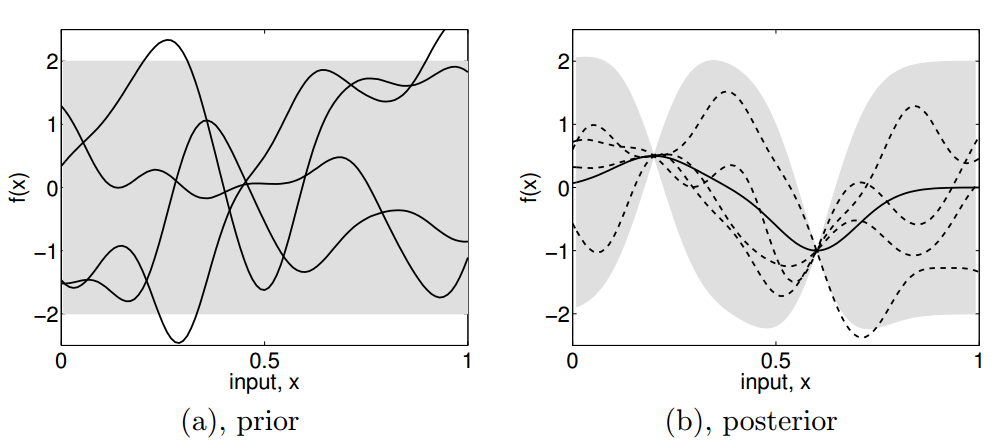
\includegraphics[scale = 0.45]{assets/GaussianProcess_2a664.png}
            \caption{Panel (a) shows four samples drawn from the prior distribution. Panel
(b) shows the situation after two datapoints have been observed. The mean prediction
is shown as the solid line and four samples from the posterior are shown as dashed
lines. In both plots the shaded region denotes twice the standard deviation at each
input value x.}
        \end{figure}
        上图是高斯过程的一个图解:
        在先验概率的条件下,采样空间有无数个多的函数可以选择,

        在后验概率的条件下,则采样的范围就会缩小

        而在高斯过程中,我们进一步把采样的范围缩小到高斯分布的范围内。

        {\color{blue}这里的函数的采样,具体地看,就是对函数的参数$\bm w$的采样,而参数也满足高斯分布,因此,参数是从高斯分布采样得到的。(具体见贝叶斯回归与高斯过程的关系)}

        \subsection{超参数的学习}
        在高斯过程中,我们抛弃参数模型,直接定义函数上的先验概率分布({\color{blue}具体表现为函数值$y_i$的概率分布}),
        而这个分布则取为高斯分布,确定一个高斯分布,只需要找到它的均值和方差即可。
            \subsubsection{均值}
            前面已经提到,在大部分应用中,我们对于函数值$y_i$的均值没有任何的先验知识,因此根据对称性,我们取均值为$0$

            \subsubsection{协方差矩阵$\bm K$}
            $\bm K$矩阵叫相似性矩阵,用来描述随机变量之间的相似性,

            i.e. 对于相似的$\bm x_n$和$\bm x_m$,对应 的函数值$y(x_n)$和$x_m$的相关性要大于不相似的点。这里相似性的概念取决于实际应用。

            对于高斯过程回归,一个广泛使用的和函数的形式为指数项的二次型加上常数项和线性项,i.e.
            \begin{equation}
                k(\bm x_n,\bm x_m) = \theta_0 exp\{-\frac{\theta_1}{2}\| \bm x_n - \bm x_m \|\} + \theta_2 + \theta_3\bm x_n^T \bm x_m
            \end{equation}

            \subsubsection{学习超参数}
            学习超参数的方法基于计算似然函数$p(\bm t|\bm \theta)$,其中$\bm \theta$表示高斯过程模型的超参数。最简单的方法是通过
            最大化似然函数的方法进行$\bm \theta$的点估计。

            使用\textbf{多元高斯分布}的标准形式,高斯过程模型的对数似然函数形式为:
            \begin{equation}
                \ln p(\bm t|\bm \theta) = -\frac{1}{2}\ln|\bm C| - \frac{1}{2}\bm t_T\bm C^{-1}\bm t - \frac{n}{2}\ln 2\pi
            \end{equation}

        \subsection{自动相关性确定 automatic relecance determination ARD}
        上一节用似然函数求参数的方法,这里我们通过为每一个输入变量整合一个单独的参数,在通过最大似然函数方法进行参数的最优化,就能够自动地将不同输入的相对重要性从数据中推断出来。

        e.g.考虑二维输入空间$\bm x = (x_1,x_2)$,有以下形式的核函数:
        \begin{equation}
            k(\bm x , \bm x') = \theta_0 exp{\frac{1}{2}\sum_{i = 1}^2\eta_i(x_i - x_i')^2})
        \end{equation}
        {\color{blue}这里的相关性,某个属性的相关性,而不是某个输入样本的相关性}

        \subsection{怎样从高斯分布中采样}

        \begin{figure}[H]\centering
            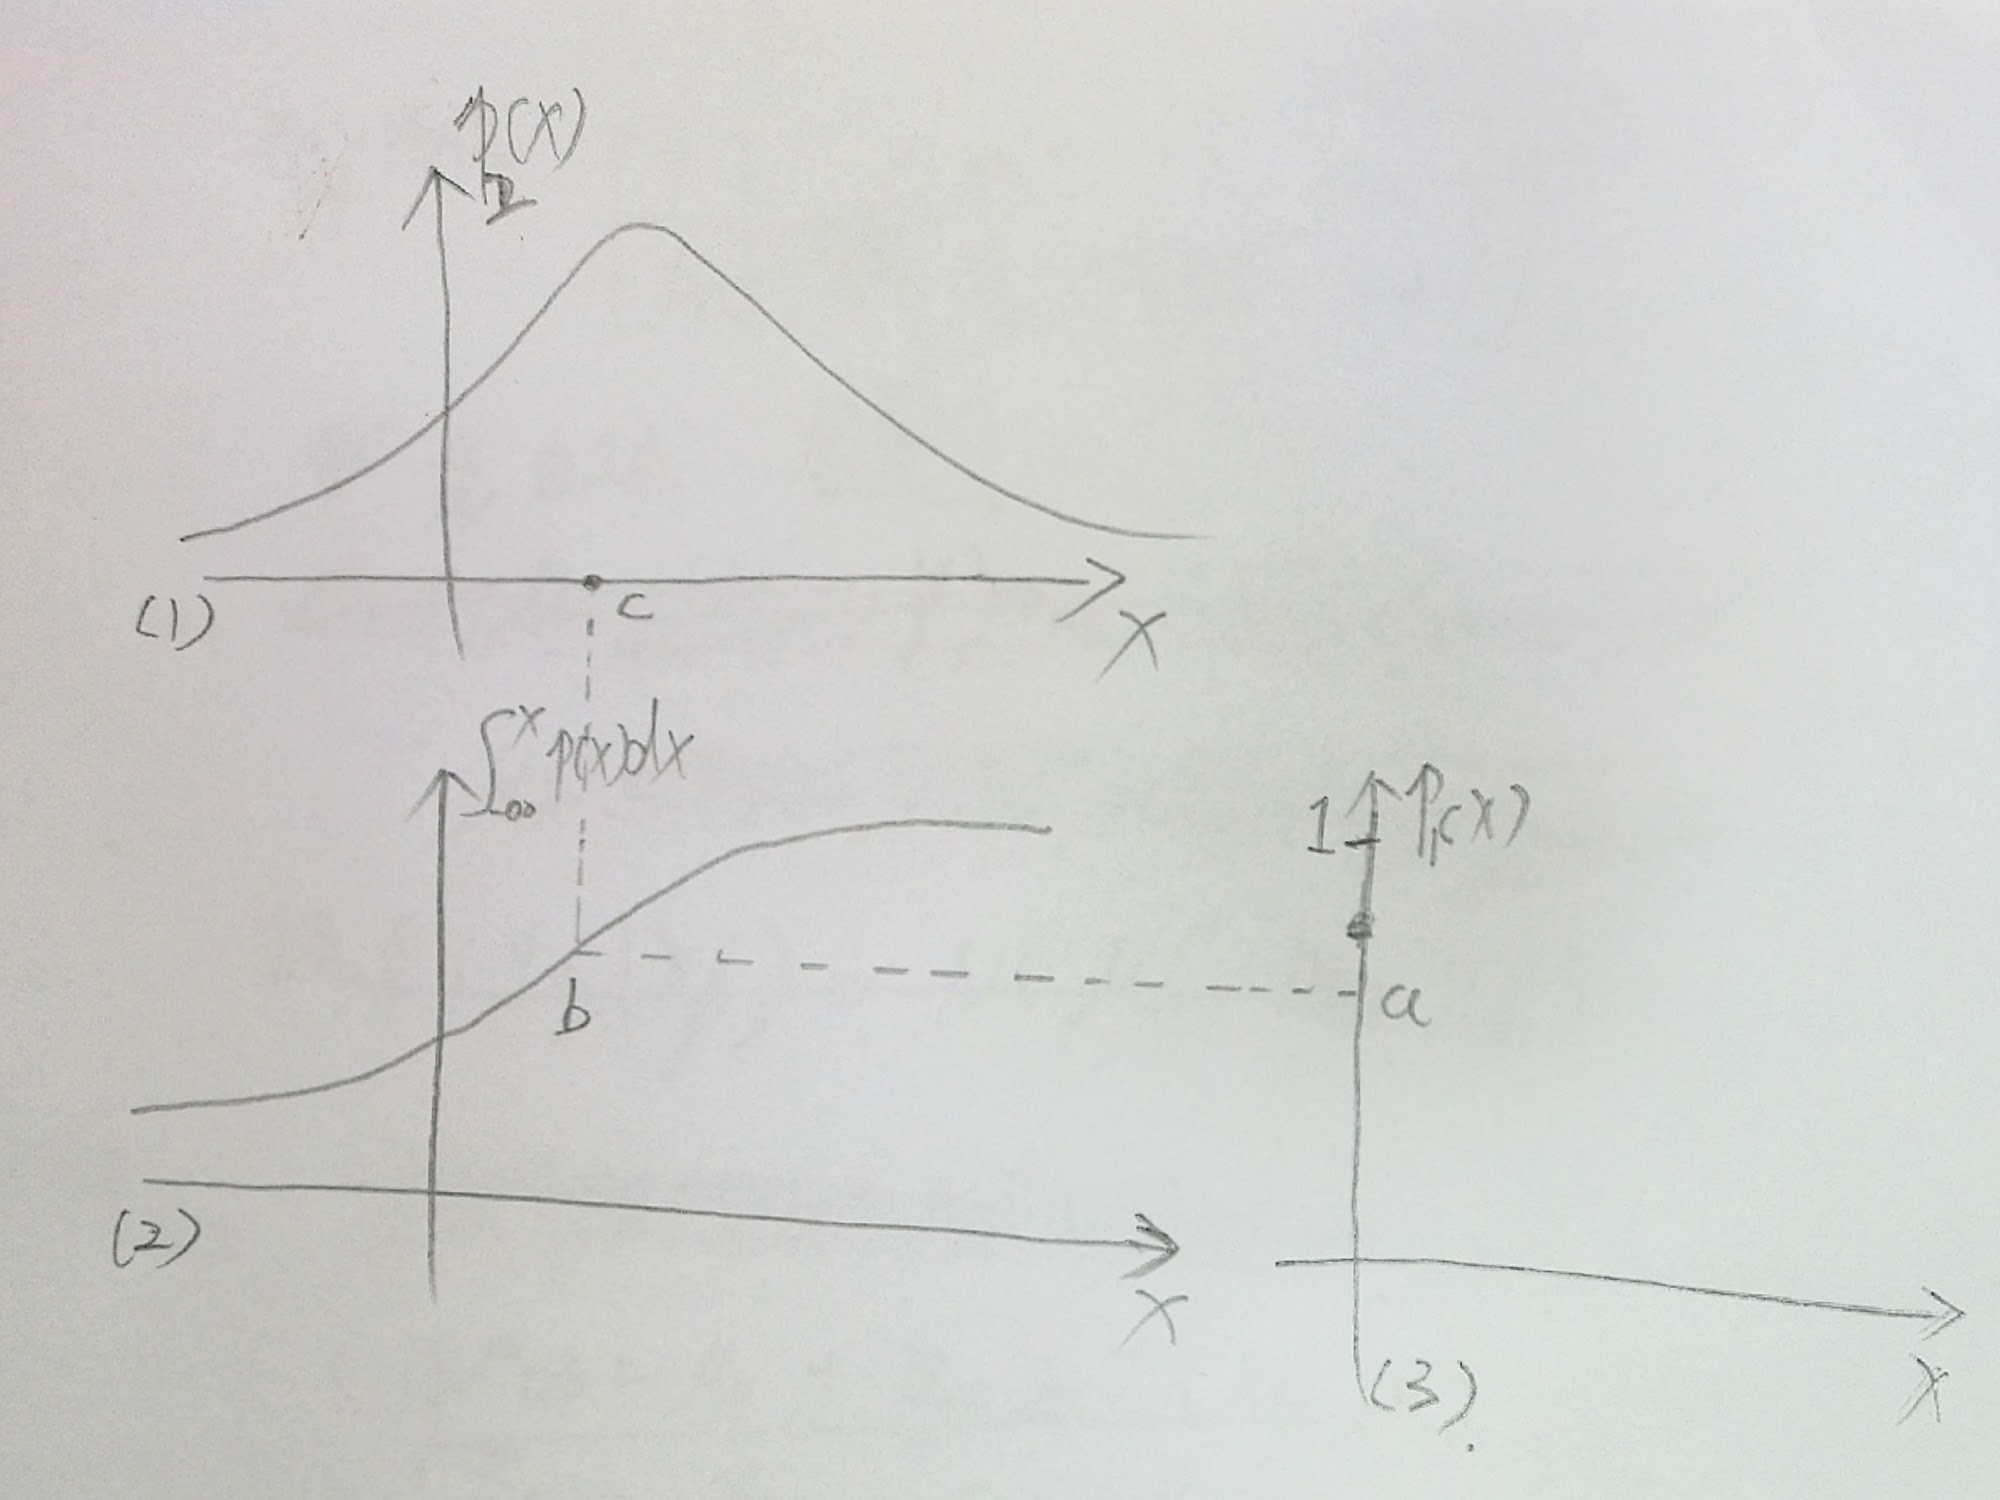
\includegraphics[scale = 0.2]{assets/GaussianProcess_16efa.png}
            \caption{(1):表示高斯分布,(2)表示从负无穷到$x$曲线下的面积,(3)表示均匀分布}
        \end{figure}
        采样过程:从(3)的均匀分布中采样得到点$a$,点$a$对应面积曲线中的点$b$,点$b$对应到高斯分布的点$c$,点$c$就是高斯分布采样的一个结果。

        \subsection{与神经网络的关系}
        在贝叶斯神经网络中,定义参数$\bm w$上的先验分布以及网络函数$f(\bm x,\bm w)$产生了函数$y(\bm x)$上的先验概率分布,其中$\bm y$表示网络的输出向量。

        在$M\to \infty $的情况下,神经网络产生的函数的分布将会趋于高斯过程。

        然而,值得注意的是,在这种期限情况下,神经网络的输出将会变得相互独立。神经网络的优势之一是输出之间共享隐含单元,因此它们可以互相"借统计优势",即,每个隐含节点关联的权值将被所有的输出变量影响,而不只是被它们中的某一个影响。这个性质在极限的高斯过程中丢失了。

        \subsection{与岭回归的关系}
        岭回归的优化目标是:
        \begin{equation}
            \min_{\bm \theta} \|\bm y - \bm X\bm \theta\| + \delta^2\|\bm \theta\|^2
        \end{equation}
        有解析解:
        \begin{equation}
            \bm \theta = \bm X^T \bm \alpha
        \end{equation}
        其中,
        \begin{equation}
            \bm \alpha = (\bm X\bm X^T + \delta^2 \bm I_n)^{-1}\bm y
        \end{equation}

        那么给定$\bm x_*$,其预测值$y_*$为:
        \begin{equation}
            y_* = \bm x_*\bm \theta = \bm x_* \bm X^T\bm \alpha = \bm x_*\bm X^T(\bm X\bm X^T + \delta^2 \bm I_n)^{-1}\bm y
                    = \bm K_*^T\bm C^{-1}\bm y
        \end{equation}
        即,最后预测的值和高斯过程中,$y_*$分布的均值是相等的。

        {\color{blue}这里体现了高斯过程的一个有点,高斯过程不仅能得到岭回归下的预测结果(均值),还能得到对于每个$y_*$预测的上下边界。}

        \subsection{与贝叶斯线性回归模型的关系}
        \textbf{贝叶斯线性回归模型:}{\color{blue}具体见PRML3.3章}
        引入$\bm w$的先验概率分布,形式为:
        \begin{equation}
            p(\bm w) = \mathcal{N}(\bm w | \bm m_0 , \bm S_0)
        \end{equation}

        在输入$\bm t$下的后验概率分布形式为:
        \begin{equation}
            p(\bm w | \bm t) = \mathcal{N}(\bm w | \bm m_N , \bm S_N)
        \end{equation}
        其中,
        \begin{equation}
            \bm m_N = \bm S_N(\bm S_0^{-1}\bm m_0 + \beta \bm \Phi^T\bm t)
        \end{equation}
        \begin{equation}
            \bm S_N^{-1} = \bm S_0^{-1} + \beta \bm \Phi_T \bm \Phi
        \end{equation}

        预测分布:{\color{blue}也是求在输入和超参的条件下,预测值的分布}
        \begin{equation}
            p(t|\bm t , \alpha ,\beta)  = \int p(t|\bm w,\beta)p(\bm w|\bm t,\alpha , \beta) d\bm  w
        \end{equation}
        预测分布的形式为:
        \begin{equation}
            p(t|\bm t , \alpha ,\beta) = \mathcal{N}(t | \bm m_N^T\bm \phi(\bm x),\sigma_N^2(\bm x))
        \end{equation}
        其中,
        \begin{equation}
            \sigma_N^2*(\bm x) = \frac{1}{\beta} + \bm \phi(\bm X)^T\bm S_N \bm \phi(\bm x)
        \end{equation}

        因此,贝叶斯线性回归模型是高斯过程的一个具体例子。

        \subsection{参考资料}
        \begin{itemize}
            \item PRML 2.3,3.35.7,6.4,8.1
            \item \href{http://www.gaussianprocess.org/gpml/}{Gaussian Processes for Machine Learning}
            \item \href{http://blog.csdn.net/jasonding1354/article/details/49818575}{【机器学习技术】高斯过程初探}
            \item \href{https://www.zhihu.com/question/46631426}{如何通俗易懂地介绍 Gaussian Process?-知乎}
            \item \href{http://blog.csdn.net/daunxx/article/details/51725086}{贝叶斯线性回归(Bayesian Linear Regression)}
            \item \href{http://www.youtube.com/watch?v=4vGiHC35j9s}{Machine learning - Introduction to Gaussian processes-UBC}
        \end{itemize}

\end{document}
